\section{Solution proposée}

\subsection{Concepts de base}
    \begin{frame}
        \frametitle{Capteurs extéroceptifs et proprioceptifs}
        \begin{columns}[c]                
            \begin{column}{0.65\textwidth}
                \begin{itemize}
                    \item \textbf{Extéroceptif} : mesure des objets relativement au robot.\vspace{6 mm}
                    \item \textbf{Proprioceptif} : mesure interne au robot.
                \end{itemize}                         
            \end{column} 
                            
            \begin{column}{0.3\textwidth}
                \begin{figure}                 
                    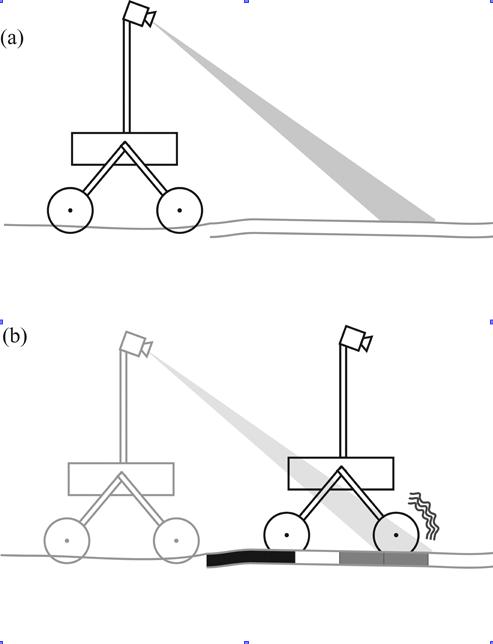
\includegraphics[width=\textwidth,height=0.6\textheight]{./media/completeSensors.png}
                \end{figure}
            \end{column}            
        \end{columns}              
    \end{frame}
    
    \begin{frame}
        \frametitle{Classement supervisé}
        \begin{columns}
            \begin{column}{0.4\textwidth}
                \vspace{-4mm}
                \begin{figure}
                    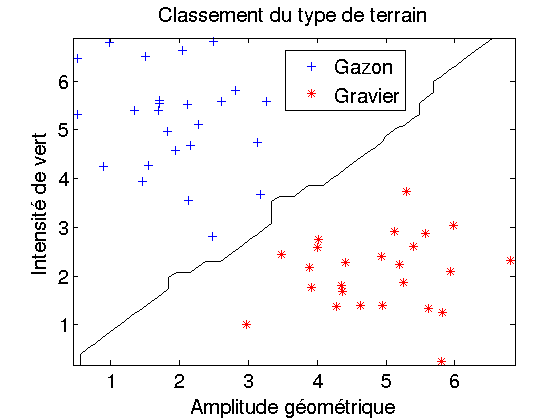
\includegraphics[width=1.2\textwidth]{./media/machineLearning.png}
                \end{figure}                   
            \end{column} 
                            
            \begin{column}{0.6\textwidth}
            \note{Échantillon-photo,feature-intensitéVert/amplituteGéometrie}
            \note{Étiquette-gazon/roches, entrainement fournir un ensemble}
                Concepts du classement :\\ \vspace{3mm}                
                \begin{itemize}
                    \item étiquette de classe
                    \item échantillon (ou exemple ou donnée)
                    \item entrainement;
                    \item caractéristiques (ou \textit{features});                         
                    \item frontière de décision.
                \end{itemize}           
            \end{column}
        \end{columns}          
    \end{frame}
    
\subsection{Solution}
    \begin{frame}[allowframebreaks]
        \frametitle{Solution proposée}
        \textbf{Classement auto-supervisé :} \\  
        \begin{itemize}
            \item un algorithme de classification permet d'identifier l'étiquette de classe d'une zone du terrain traversée par le robot grâce aux capteurs proprioceptifs;
            \item les étiquettes ainsi obtenues permettent d'entrainer un classifieur utilisant les données des capteurs extéroceptifs.
        \end{itemize} 
    \end{frame}
    
    \begin{frame}[c]
        \begin{columns}[c]
            \begin{column}{0.4\textwidth}
                \begin{figure}
                    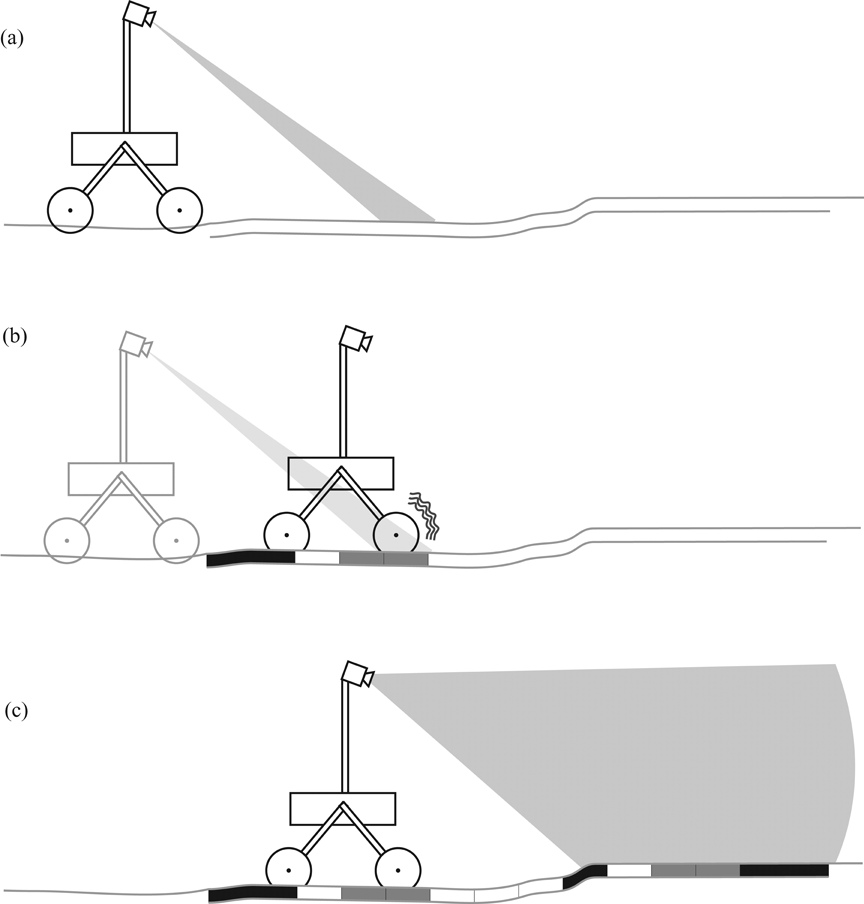
\includegraphics[width=\textwidth]{./media/selfSupervised.png}
                \end{figure}            
            \end{column}
            
            \begin{column}{0.6\textwidth}
            Avantages : \\ \vspace{1mm}
                \begin{itemize}
                    \item élimine une étape d'étiquetage manuelle ;
                    \item l'apprentissage par expérience est adaptatif.
                \end{itemize}
            \end{column}
        \end{columns}         
    \end{frame}
    